
\begin{figure}[ht]
\begin{subfigure}{\textwidth}
\centering
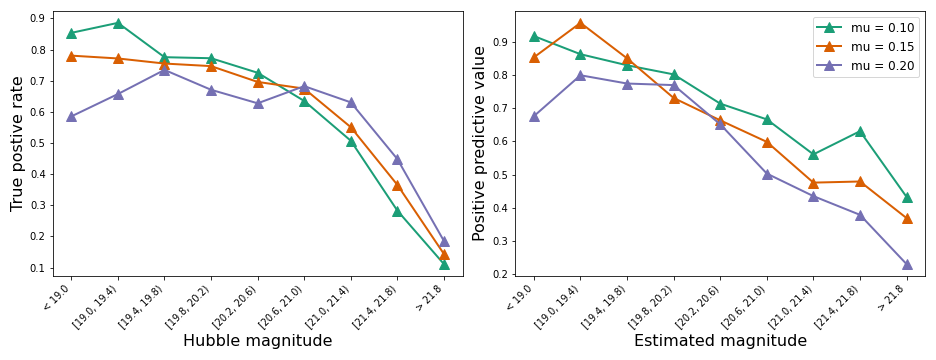
\includegraphics[width = \textwidth]{figures/prior_mu_sensitivty.png}
\end{subfigure}
\begin{subfigure}{\textwidth}
\begin{center}
\begin{tabular}{rrr}
\toprule
     mu &   TPR &   PPV \\
\midrule
 1000&  0.49 &  0.69 \\
 1500&  0.49 &  0.64 \\
 2000 &  0.52 &  0.49 \\
\bottomrule
\end{tabular}
\par\vspace{0pt}
\end{center}
\end{subfigure}\hfill
\caption{Sensitivity of summary statistics to Poisson mean parameter on number of stars. }
\end{figure}

\begin{figure}[ht]
\begin{subfigure}{\textwidth}
\centering
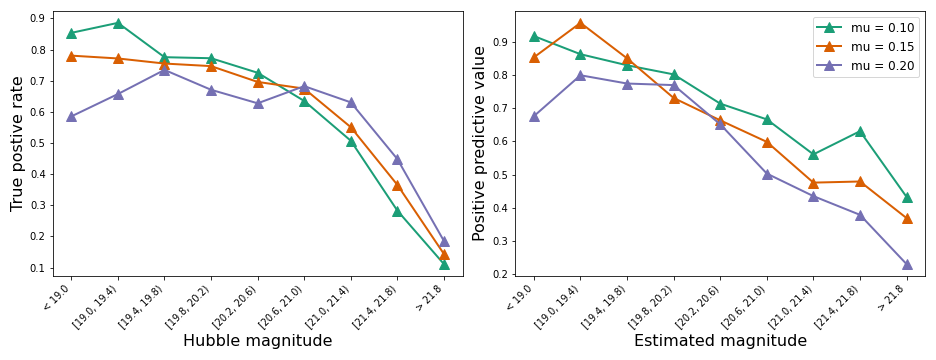
\includegraphics[width = \textwidth]{figures/prior_mu_sensitivty.png}
\end{subfigure}
\begin{subfigure}{\textwidth}
\begin{center}
\begin{tabular}{rrr}
\toprule
     mu &   TPR &   PPV \\
\midrule
 1000&  0.49 &  0.69 \\
 1500&  0.49 &  0.64 \\
 2000 &  0.52 &  0.49 \\
\bottomrule
\end{tabular}
\par\vspace{0pt}
\end{center}
\end{subfigure}\hfill
\caption{Sensitivity of summary statistics to Poisson mean parameter on number of stars. }
\end{figure}
